\documentclass{article}
\usepackage{preamble}

\begin{document}

\maketitle

\section{Introduction}

Prediction markets can be used to elicit and aggregate agents' information about some event \cite{conitzerPredictionMarketsMechanism2012, hansonLogarithmicMarketScoring2002, hansonCombinatorialInformationMarket2003}; for example, the market price for the contract ``Pays \$1 if a Republican wins the 2024 US Presidential Election'' can be interpreted as the probability assigned by the market to the event that a Republican wins the 2024 US Presidential Election (we will make this notion precise in subsequent sections).

On the surface, prediction markets seem to solve basically every problem in your life: any question, any difference of opinion, even any scientific question, is optimally addressed by simply setting up a prediction market for it, yielding the single best probability estimate as an answer from all information present in the world. 

Closer inspection reveals a fundamental limitation of prediction markets: they can only elicit probabilities for sentences that are either \emph{verifiable} (if true, then will be revealed true -- e.g. ``there exists a white swan'') or \emph{falsifiable} (if true, then will be revealed false -- e.g. ``all swans are white''). However, intelligent agents generally hold beliefs about a much wider class of sentences: sentences that only hold meaning in an agent's mental model, that could be described as ``sentences that are neither verifiable nor falsifiable (non-VF)'', ``beliefs in the latent space'' or even ``subjective beliefs''.

\begin{figure}
    \centering
    \usetikzlibrary{arrows}
\usetikzlibrary{positioning}
\pgfmathsetmacro{\myw}{3.6}
\pgfmathsetmacro{\myh}{2.6}
\pgfmathsetmacro{\mys}{0.25}
\newlength{\mypad}
\setlength{\mypad}{8pt}
\newlength{\mylsg}
\setlength{\mylsg}{2pt}

\begin{tikzpicture}[line width =1pt]

\draw (0,0) -- (0,3*\myh+4*\mys);
\draw (\myw,0) -- (\myw,3*\myh+4*\mys);
\node[] at (\myw/2,3*\myh+4*\mys){$\dots$};
\draw node[above = \mypad, anchor = north east]{$\Delta_0$} (0,0) -- (\myw,0) node[above = \mypad, anchor = north west]{$\Delta_0$};
\draw (0,0) -- (\myw,\myh) node[above = \mypad, anchor = north west]{
    \begin{tabular}{l}
        $\Pi_1$ \vspace{\mylsg}\\
        ``Bob will die'' \vspace{\mylsg}\\
        ``all swans are white'' \vspace{\mylsg}\\
        ``$P$ does not halt''
    \end{tabular}};
\draw (\myw,0) -- (0,\myh) node[above = \mypad, anchor = north east]{
    \begin{tabular}{r}
        $\Sigma_1$ \vspace{\mylsg}\\
        ``Bob will die'' \vspace{\mylsg}\\
        ``there is a white swan'' \vspace{\mylsg}\\
        ``$P$ halts''
    \end{tabular}};
\draw (0,\myh+\mys) -- (\myw,2*\myh+\mys) node[above = \mypad, anchor = north west]{
    \begin{tabular}{l}
        $\Pi_2$ \\
        ``all men are mortal'' \vspace{\mylsg}\\
        ``all swans will lay\\
        a white egg'' \vspace{\mylsg}\\
        ``there are an infinite\\
        number of primes''
    \end{tabular}};
\draw (\myw,\myh+\mys) -- (0,2*\myh+\mys) node[above = \mypad, anchor = north east]{
    \begin{tabular}{r}
        $\Sigma_2$ \\
        ``there is an immortal man'' \vspace{\mylsg}\\
        ``there is a swan that\\
        always lays brown eggs'' \vspace{\mylsg}\\
        ``there are finitely\\
        many perfect numbers''
    \end{tabular}};
\draw (0,2*\myh+2*\mys) -- (\myw,3*\myh+2*\mys) node[above = \mypad, anchor = north west]{
    \begin{tabular}{l}
        $\Pi_3$ \vspace{\mylsg}\\
        ``$x_n$ converges to 2''
    \end{tabular}};
\draw (\myw,2*\myh+2*\mys) -- (0,3*\myh+2*\mys) node[above = \mypad, anchor = north east]{
    \begin{tabular}{r}
        $\Sigma_3$ \vspace{\mylsg}\\
        ``$x_n$ does not converge to 2''
    \end{tabular}};
\end{tikzpicture}
    \caption{The ``arithmetical hierarchy'' of FOL sentences. A $\Sigma_{n+1}$ sentence is of the form $\exists x,p(x)$ where $p$ is $\Pi_n$; a $\Pi_{n+1}$ sentence is of the form $\forall x,p(x)$ where $p$ is $\Sigma_n$. In logic, the lowest level of the arithmetical hierarchy $\Delta_0=\Sigma_0=\Pi_0$ are sentences of the form $f(n)=0$ where $f$ is a primitive recursive function, but this formalism may be extended to empirical truths that will be revealed at a fixed time}
    \label{fig:fol}
\end{figure}

One type of such a class of sentences is sentences expressible in some logic, e.g. First-Order Logic (FOL), as in Fig~\ref{fig:fol}. But even this does not capture the full scope of sentences in an agent's latent space: e.g. claims about events in the past, claims about a tree falling in the forest with no one to hear it, claims about quarks, claims about hypotheticals that will certainly never be carried out, vaguely-specified claims. 

One approach to dealing with such sentences, which could be said to be the philosopher's approach, is to reject non-VF sentences as meaningful at all. However, we may defend such sentences on the basis of their practical value: take the sentence ``Bob is guilty''. This sentence in itself is non-VF; however, it is \emph{correlated} with other, directly empirical or practically valuable sentences such as ``If we release Bob from prison, he will commit more crimes'' and ``we will find blood in Bob's house'': intuitively, we expect that agents, seeing a high price for ``Bob is guilty'', will also bid up ``we will find blood in Bob's house'', or bid against releasing Bob on a decision market. Thus ``Bob is guilty'' can be seen as a latent space variable that captures correlations between different variables. This is expounded on in \cite{tailcalledLatentVariablesPrediction2023}.

\begin{goals*}
    Broadly speaking, I seek to \emph{create market-based mechanisms for creating and betting on latent space variables}. More precisely, this can be expressed in terms of two slightly differing research questions:
    \begin{enumerate}
        \item (As a toy model) How can we develop markets that meaningfully price sentences expressible in FOL (or more generally any hyperarithmetical logic)? 
        \item How can we develop markets that decide (with the objective of maximizing some utility function) what kind of latent space to build, and then elicit bets on questions in the latent space?
        \item How can we develop prediction markets that incentivize a collection of agents to develop ``mutually interpretable'' latent spaces, i.e. such that they can cheaply and honestly place bets on sentences framed in each other's latent spaces with good calibration and scores.
    \end{enumerate}
\end{goals*} 

\begin{work*}
    I've addressed RQ 1 in my draft paper \cite{abhimanyupallavisudhirBettingWhatNeither2023} and produced a framework for betting on FOL sentences; I'll elaborate on the precise framework in subsequent sections.
\end{work*}

\begin{applications*}
    Besides the obvious utility of constructing prediction markets for arbitrary subjective sentences, the primary application of my work is to \emph{AI alignment}. More precisely:
    \begin{itemize}
        \item The desiderata outlined above for my market-based mechanism -- forming a latent space that captures patterns in observed data -- are essentially identical to the function of an intelligent agent. My hope therefore is that my research could lead to an alternate, market-based framework for AI agents, and there are intuitive reasons to expect such a framework to be immune to many forms of misalignment.
        \item Eliciting bets on latent space knowledge, if robust frameworks to incentivize this are developed, have been identified as an approach to AI interpretability \cite{christianoElicitingLatentKnowledge2021}. 
\end{itemize}
\end{applications*}

%% bounded rationality -> this

\section{Literature survey}

\subsection{Prediction markets}

We will describe the general setting of a basic prediction market, specifically under the Logarithmic Market Scoring mechanism of \cite{hansonCombinatorialInformationMarket2003, hansonLogarithmicMarketScoring2002} as that framework is most natural for simultaneously addressing \emph{which questions should prediction markets be created for}, etc.

\begin{definition}[Finite process]
    A ``finite process'' $X$ is the tuple of a resolution time $X.t\in\Nats$, and a true value $X.x\in\Bools$ (which may be sampled from some probability distribution at time $t$).
    \label{def:finproc}
\end{definition}

We concern ourselves with some particular set $\finprocs$ of finite processes, e.g. statements of the form $f(n)=0$ where $f$ is a primitive recursive function over the natural numbers and the resolution time is given by some enumeration of the primitive recursive functions. In particular $\finprocs$ should contain elements $\top$ and $\bot$ which have resolution time $t=0$ and true value $v=1$ and $0$ respectively. Furthermore we denote the type of finite-supported maps $\finprocs\times\Bools\too\Rats$ as $\portfolios$ (for ``portfolio''). 

\begin{definition}[Agent]
    An ``agent'' $\agent$ is a computable function $\trader:\Nats\to\portfolios$ paired with a ``starting endowment'' $\endowment\in\Rats$. [Here, $\trader(t)$ should be interpreted as the order submitted by the agent, i.e. which should get added to its portfolio if all goes well]
    \label{def:agent}
\end{definition}

Again, we concern ourselves with some particular class $\agent[s]$ of agents and specifically a surjective ``enumerator'' of agents $\father:\Nats\to\agent[s]$ such that $\sum_{t\in\Nats}\endowment[\father(t)]<\infty$ that allows us to have a potentially infinite number of traders that are gradually added to trade in the market.

\begin{definition}[Classic prediction market]
    A prediction market for a finite process $X$ is defined by a ``costing function'' $P:\portfolios\to\Reals$ and the following procedures for updating each agent's inventory $\inventory:\portfolios$ (note that in particular, $\inventory(\top,\top)$ is interpreted as $\agent$'s cash reserves) and market prices $\pricee:\finprocs\times\Bools\to\probs$:
    \begin{algorithm}
    \begin{algorithmic}
    \Function{Rewarder}{}
        \For{$t\in\Nats$}
            $\inventory[\father(t)](\top,\top)\gets\endowment[\father(t)]$
            \For{$\agent\in\{\father(0),\dots\father(t)\}$}
                \For{$X\in\supp{\inventory}$} \Comment{for all stocks $\agent$ has a stake in}
                    \If{$t\ge X.t$} \Comment{if they're resolved}
                        \State $\inventory(\top,\top)\gets \inventory(X, X.x)$ \Comment{convert them into cash}
                        \State $\inventory(X,\top)\gets 0$
                        \State $\inventory(X,\bot)\gets 0$
                    \EndIf
                \EndFor
            \EndFor
        \EndFor
    \EndFunction
    \Function{Market}{}
        \State $\inventory[p]\gets\mathbf{0}$ \Comment{initialize total count of stocks in circulation}
        \For{$t\in\Nats$}
            \For{$\agent\in\{\father(0),\dots\father(t)\}$}
                \State $\Delta\inventory \gets \agent(t)$ \Comment{input trade order}
                \State $\Delta\inventory(\top,\top) \gets P(\inventory)-P(\inventory+\Delta\inventory)$ \Comment{calculate order cost}
                \If{$\inventory(\top,\top)+\Delta\inventory(\top,\top)\ge 0$}\Comment{Check if in budget}
                    \State $\inventory\gets\inventory+\Delta\inventory$
                    \State $\inventory[p]\gets\inventory[p]+\Delta\inventory$
                \EndIf
                \State $\pricee\gets\nabla P(\inventory[p])$
            \EndFor
        \EndFor
    \EndFunction
    \end{algorithmic}
    \end{algorithm}
    \label{def:predmarket}
\end{definition}

The above definition is for some general ``costing function'' $P$ whose gradient is the instantaneous price: in general, any costing function corresponds to a \emph{scoring rule}: if you push the price of some asset from $\pricee$ to $\pricee'$ with your trades, and that asset resolves to $\top$, your profit can be described as a score $s(\pricee')-s(\pricee)$ you receive for your prediction. More precisely, and slightly generalizing the statement in \cite{hansonLogarithmicMarketScoring2002, hansonCombinatorialInformationMarket2003}:

\begin{definition}[Corresponding scoring rule]
    A necessary condition for an acceptable costing function is that $\nabla P(\inventory[m]')=\nabla P(\inventory[m])$ only when $\inventory[m]'-\inventory[m]$ amounts to a cash term (i.e. an equal distribution over all mutually exclusive stocks), and that in this case $P(\inventory[m]')-P(\inventory[m])=\inventory[m]'-\inventory[m]$. In that case, the costing function leads to a scoring rule for report $\pricee$ given by $s(\pricee)=\theta(\pricee)-P\circ\theta(\pricee)$ where $\theta$ is any right-inverse of $\nabla P$, i.e. $\theta(\pricee)$ is a portfolio that leads to a market price of $\pricee$. 
    \label{def:scoring}
\end{definition}

With this, all the standard textbook knowledge about scoring rules can be applied (indeed this was the central insight of \cite{hansonLogarithmicMarketScoring2002, hansonCombinatorialInformationMarket2003}). For instance, we would like a costing function such that its corresponding scoring rule is \emph{proper}, i.e. if $\Expect[s(\mathbf{r})]$ is maximized under a probability distribution $\pricee:\finprocs\to\probs$ when $\mathbf{r}=\pricee$. 

The choice of this costing function determines the mechanism, and can generally be interpreted as expressing \emph{how the market-maker demands information}. For instance, under \emph{logarithmic market scoring}, the market maker is essentially paying a linear cost for information on some finite process, i.e. some price per bit of information on $X$. More precisely:

\begin{definition}[Logarithmic Market Scoring (LMSR)]
    Logarithmic market scoring \cite{hansonLogarithmicMarketScoring2002} is defined by the costing function:
    
    \begin{equation*}
        P(\inventory) = \sum_{X\in \supp{\inventory}}{\lambda_X\log
        \sum_{x\in\Bools}{\exp\left(\inventory(X, x)/\lambda_{X}\right)}}
    \end{equation*}
    
    Where $\lambda_X$ the ``market-maker subsidy'' for the market on $X$ (if the finite processes can be computably enumerated, $\lambda_X$ can be pre-specified so it sums to a finite value over all $X$). In fact it represents the price per bit of information on the value of $X$. One can check that prices are then given by:
    
    \begin{equation*}
        \nabla P(\inventory, X, x) = \frac{\exp\left(\inventory(X, x)/\lambda_{X}\right)}{\sum_{x\in\Bools}{\exp\left(\inventory(X, x)/\lambda_{X}\right)}}
    \end{equation*}
    
    One may check that the resulting scoring rule (the total market payout made in each possible outcome, for moving prices to $\mathbf{r}$) is $\mathbf{s}(\mathbf{r})=\left[\lambda_{X}\log\mathbf{r}(X, x)\right]_{X\in\finset{\finprocs}, x\in\Bools}$, the expectation of which, under belief $\pricee$, is:
    
    \begin{equation*}
        s(\pricee, \mathbf{r})
        =\sum_{X}\sum_{x\in \Bools}\lambda_{X}\pricee(X, x)\log\mathbf{r}(X, x)=-\sum_{X}\lambda_{X}H(\pricee(X), \mathbf{r}({X}))
    \end{equation*}
    
    Thus the expected profit from making a report $\mathbf{r'}$ when current market prices are $\mathbf{r}$:
    
    \begin{equation*}
        \Delta s(\pricee, \mathbf{r}, \mathbf{r}') = s(\pricee, \mathbf{r}') - s(\pricee, \mathbf{r}) = \sum_{X} \lambda_{X}\left[H(\pricee({X}), \mathbf{r}({X})) - H(\price({X}), \mathbf{r}'({X}))\right]
    \end{equation*}
    
    Where $H$ is cross-entropy. We would \emph{like} to say that $\Delta s(\pricee, \mathbf{r}, \mathbf{r}')$ is maximized when $\mathbf{r}'=\pricee$, but the report $\mathbf{r}'$ has finite support while $\pricee$ is not, so there is no ``best possible report'' to make. But we can see that the profit is decreasing in the cross-entropy $H(\pricee(X), \mathbf{r}'({X}))$, i.e. the closer your report to your true belief, the better.
    \label{def:lmsr}
\end{definition}

\subsection{Program markets}

We will describe here, in brief, two existing works in the literature describing ``program markets'', i.e. markets whose participants are taken to be programs rather than some utility-maximizing agents. Treating the market as a whole as an aggregate agent then quite nicely captures a notion of bounded rationality, because a market can be understood as being optimally rational \emph{as constrained by the algorithmic information (i.e. programs) available to it}. 

The first work we will describe is \cite{garrabrantLogicalInduction2016}, a framework for logical uncertainty, to which my work \cite{abhimanyupallavisudhirBettingWhatNeither2023} can be seen as a competing framework. The work defines a prediction market for all logical sentences which pays off whenever a sentence is proven by some formal theorem prover (which exists for any ``computably enumerable theoory'', including first-order arithmetic etc.). However, as stated, this would simply be a prediction market for the \emph{provability} of a sentence (in some particular formal theory); the actual Garrabrant induction framework instead adopts a notion of ``propositionally consistent worlds'' that allows even unprovable (and provably unprovable) sentences to have non-zero probabilities and such that basic probabilistic laws like $\Prob(P)+\Prob(\lnot P)=1$ are followed.

The idea is as follows: if $P\lor Q$ is proven, then an agent that holds a stock each in sentences $P$ and $Q$ must necessarily be regarded as having \emph{at least} \$1 between these assets. Similarly if $\lnot P\lor\lnot Q$ is proven, then that agent has \emph{at most} \$1 between these assets. We call these different logical possibilities ``worlds'' or rather ``worlds that are propositionally consistent with the output of the theorem prover so far'' (PC worlds for short). In particular when evaluating whether a trade is within budget (to be accepted by the market-maker), we demand that it is within budget in all PC worlds. More precisely:

\begin{definition}[Worlds and valuations]
    Let $\inventory:\Props\too\Rats$ be a finite-supported map, and let $\world:\Props\to\Bools$ be a \emph{world}, i.e. a truth-assignment, so the dot product $\world\cdot\inventory$ represents the valuation of $\inventory$ according to $\world$.
\end{definition}

\begin{definition}[PC worlds]
     A world is said to be propositionally consistent (PC) if for all $P\in\Props$, $\world(P)$ is determined by Boolean algebra from the prime sentences in $\Props$, i.e. $\world(P\land Q)=\world(P)\land \world(Q)$, $\world(P\lor Q)=\world(P)\lor \world(Q)$, etc. Furthermore, let $\thms_t$ be the subset of $\Props$ proven by time $t$: then a world is said to be PC with $\thms_t$ if (1) it is PC and (2) $\world(P)=1$ for all $P\in\thms_t$. We denote the set of worlds PC with $\thms_t$ as $\PC(\thms_t)$; in particular $\PC:=\PC(\{\})$. For any $\inventory$, denote its set of plausible valuations as $\PC(\thms_t,\inventory):=\{\world\cdot\inventory\mid \world\in\PC(\thms_t)\}$.
\end{definition}

Note that $\PC(\thms_t,\inventory)$ is computable, since you only have to check propositional consistency for the sentences actually supported by $\inventory$. 


Another quirk of Garrabrant induction is that agents have type $\agent:\Nats\to(\Props\to\probs)\to(\Props\to\Rats)$ i.e. they output ``joint'' demand schedules allowing for cross-elasticity of demand rather than leaving this to be figured out by the market dynamics. Naturally, calculating equilibrium between such demand schedules is non-trivial and requires Brouwer's fixed point theorem, as well as constraints on $\agent$ (specifically that $\agent(t)$ is continuous in price and comprised only of some particularly simple expressions depending only on some external information like price history). The framework actually implements a rational approximation of the equilibrium computed via a brute-force Farey enumeration of all rational numbers.

\begin{definition}[Garrabrant induction]
    Fix a language $\Props$, a theorem enumerator $\thms:\Nats\to\finset\Props$ (obeying in particular $s\le t\implies\thms_s\subseteq\thms_t$) and enumerator of agents $\father:\Nats\to\agent[s]\times\Rats$ such that $\father_1$ is bijective and $\sum_t\father_2(t)<\infty$ (where $\father=(\father_1,\father_2)$ and $\agent[s]$ is the type specified earlier $\Nats\to(\Props\to\probs)\to(\Props\to\Rats)$). Then the Garrabrant induction algorithm is given by the following mutual recursion:
    \begin{itemize}
        \item an ``aggregate trader'' $$\agent[m](t,\pricee):=\sum_{\agent\in\{\father(1)\dots\father(t)\}}\indicate{\min\PC(\thms_t,\inventory(t,\pricee) + \agent(t,\pricee))\ge 0}\agent(t,\pricee)$$ where $\indicate{}$ denotes an indicator function
        \item an ``equilibrium price'' $\pricee(t)$, which approximates a zero of $\agent[m](t)$ i.e. so that $\agent[m](t,\pricee(t))\approx 0$ (in particular the error should be $\le 1/2^t$)
        \item an inventory account $\inventory(t,P)$, as computed by the following algorithm:
    \end{itemize}
    
    \begin{algorithm}
    \begin{algorithmic}
    \Function{$\inventory$}{$\tau$}
        \For{$t\le\tau$}
            \State $\inventory[\father_1(t)](\top)\gets\father(t)_2$
            \For{$X\in\supp{\inventory}$} \Comment{resolve proven sentences}
                \If{$X\in\thms_t$}
                    \State $\inventory(\top) \gets \inventory(\top)+\inventory(X)$
                    \State $\inventory(X)\gets 0$
                \EndIf
            \EndFor
            \For{$X\in\supp\agent$}
                \If{$\min\PC(\thms_t,\inventory(t,\pricee) + \agent(t,\pricee))\ge 0$}
                    \State $\inventory\gets\inventory+\agent(t)$ \Comment{add trade to inventory}
                \EndIf
            \EndFor
        \EndFor
        \State \Return $\inventory$
    \EndFunction
    \end{algorithmic}
    \end{algorithm}
    \label{def:garrabrant}
\end{definition}

[A slight difference in the formulation we have presented is that we put the onus on the individual agents to calculate and include the cash payment within their orders, and the aggregate agent just zeroes their trade if they submit an invalid trade; this makes no difference to the whole algorithm.]

\begin{theorem}[Inexploitability]
    With definitions as in Def~\ref{def:garrabrant}, \emph{no trader $\agent\in\agent[s]$ can exploit the price sequence $\pricee$}, i.e. $\PC(\thms_t,\inventory(t))$ remains bounded from above. 
    \label{thm:garrabrant}
\end{theorem}

\begin{hproof}
    If any trader could exploit the price sequence, so could the aggregate trader $\agent[m]$ (as whichever trader exploits the market would also grow its proportion of $\agent[m]$'s trades to $+\infty$, and no trader can run $\agent[m]$'s finances to $-\infty$ since it would just go bankrupt). However, $\agent[m]$ cannot exploit $\pricee$ as it is set to be (arbitrary close to) an equilibrium for $\agent[m]$.
\end{hproof}

This illustrates a more general principle: markets ``dominate'' (i.e. are eventually at least good as) all of their traders. Thus a market can be regarded as a learning mechanism. 

The second work we will describe is Oesterheld's framework for ``boundedly rational agents'' \cite{oesterheldTheoryBoundedInductive2023}, which, on its surface, seems to address my entire research problem: it constructs an agent that acts in a way that is ``boundedly rational'', specifically in the setting of a decision problem. A sketch of the construction is as given by Def~\ref{def:dp}.

\begin{definition}[The problem setting]
    A decision-problem $\DP$ is some finite set of ``choices''; we deal with a decision-problem sequence $\DP(1),\DP(2),\dots$, an agent that is a sequence of choices $x(t)\in\DP(t)$ and rewards $r(t)\in[0,1]$ -- all of these, including the decision-problem sequence itself, can depend on one another via mutual recursion.

    The specific agent type we are concerned with is an \emph{estimating agent} comprised both of a sequence of \emph{choices} $\choice(t)$ and a sequence of \emph{reward estimates} $\estimate(t)\in[0,1]$. In particular we have a class of estimating agents called ``hypotheses'' $\hyps$, which could e.g. be all polynomial-time estimating agents or all $O(g(t))$-time estimating agents for some non-decreasing $g(t)$: these will be our ``traders''.
    \label{def:dp}
\end{definition}

Define an ``allowance function'' $\father:\Nats\times\hyps\to\Rats$ so that $\father(t,\hyp)$ is interpreted as the budget allocated to hypothesis $h$ at time $t$, satisfying the following properties: (1) for each $t$, only $\father(t)$ has finite support (i.e. is non-zero for only finitely many $\hyp$) (2) each hypothesis gets an infinite total allowance i.e. $\sum_t\father(t,\hyp)=\infty$ for all $\hyp$ (3) the allowance distributed per round must approach zero $\sum_{\hyp} \father(t,\hyp)\to 0$.

\begin{definition}[Oesterheld agent]
    The boundedly rational ``estimating agent'' can then be constructed as an auction conducted among all hypotheses, as described by the function $\agent[m]$ that follows.
    \begin{algorithm}
    \begin{algorithmic}
        \Function{$\agent[m]$}{}
            \State $\inventory[\hyp]\gets 0$ \Comment{for all $\hyp\in\hyps$}
            \For{$t\in\Nats$}
                \State $(\hyp_*,\estimate[\hyp]_*)\gets\argmax_{\hyp\in\hyps}\min(\estimate[\hyp](t), \inventory[\hyp])$ \Comment{pick highest bidder}
                \State $(\choice(t),\estimate(t))\gets (\hyp_*,\estimate[\hyp]_*)$ \Comment{and listen to him}
                \State $\inventory[\hyp_*]\gets \inventory[\hyp_*] + r(t)-\estimate[\hyp]_*$ \Comment{pay reward, deduct bid}
                \For{$\hyp\in\hyps$}
                    \State $\inventory[\hyp]\gets\inventory[\hyp]+\father(t,\hyp)$ \Comment{give allowance}
                \EndFor
            \EndFor
        \EndFunction
    \end{algorithmic}
    \end{algorithm}
    \label{def:oesterheld}
\end{definition}

The paper then goes on to show some analogous domination results: that $\estimate$ is not consistently an overestimate (it may still be an underestimate, because the hypotheses are bounded by their wealth) and that every hypothesis that submits the highest estimate is tested an infinite number of times.  Its key limitation, of course, is that implementing this algorithm is hopelessly intractable unless we restrict $\hyps$ to be a class of trained machine learning models (in which case it wouldn't really play the fundamental role in intelligence we would like it to).

Fundamentally similar models to \cite{oesterheldTheoryBoundedInductive2023} are found in \cite{baumModelIntelligenceEconomy1999, changDecentralizedReinforcementLearning2020, kweeMarketBasedReinforcementLearning2001}: in brief, \cite{baumModelIntelligenceEconomy1999} constructs an agent called the ``Hayek machine'' which specifically performs an Oesterheld-like algorithm in a ``Block World'' game; \cite{changDecentralizedReinforcementLearning2020,kweeMarketBasedReinforcementLearning2001} implement similar algorithms in a Reinforcement Learning setting and for worlds described by partially observable Markov Decision Processes respectively. I have not read these papers in detail yet, as I only recently learned of them, but will do so subsequently.

\subsection{Latent space prediction markets}

Finally we discuss \cite{tailcalledLatentVariablesPrediction2023}, which raises precisely the question of latent variable prediction markets. The framework proposed is very straightforward: suppose $X_1,\dots X_n$ are some correlated random variables (e.g. ``Economic metric $i$ will be good''). Then ``we'' create a latent variable $Y$, say with some natural language description (``The economy will be good''). Users can then submit bids either on $\Prob[Y]$ directly or on the distribution $\Prob[X_i|Y]$. $Y$ itself will never be revealed, but the distribution $\Prob[X_i]$ can be inferred from these distributions, and bettors are then scored based on their implied bet on this, i.e. proportional to $\log \Prob[\vec{x}]-\log \Prob_0[\vec{x}]$.

\begin{figure}
    \centering
    \usetikzlibrary{arrows}
\usetikzlibrary{positioning}

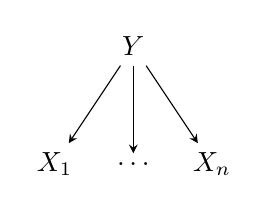
\begin{tikzpicture}[>=stealth]
    \node (Y) at (0,0) {$Y$};
    \node (X1) [below of=Y, node distance=1.5cm, xshift=-1cm] {$X_1$};
    \node (Xdots) [below of=Y, node distance=1.5cm, xshift=0cm] {$\dots$};
    \node (Xn) [below of=Y, node distance=1.5cm, xshift=1cm] {$X_n$};
    
    \draw[->] (Y) -- (X1);
    \draw[->] (Y) -- (Xdots);
    \draw[->] (Y) -- (Xn);
\end{tikzpicture}
    \caption{Causal diagram illustrating a latent variable}
    \label{fig:latent}
\end{figure}

Fig~\ref{fig:latent} illustrates the idea: postulating a latent $Y$ constrains the space of possible joint distributions $\Prob[X_1,\dots X_n]$ to only those that can be factored as $\sum_y{\Prob[X_1|Y=y]\dots\Prob[X_n|Y=y]\Prob[Y=y]}$ for some suitable $Y$. This incentivizes traders to choose good latents and bet correctly on them.

However, this formalism retains several limitations: it does not specify \emph{how} to determine which variables to specify a latent between, the specific choice of latent is maintained only by Schelling point inertia (at least in the absence of ``whale'' traders, which I suspect would create incentives for strategic behaviour), and it is not clear how to handle scenarios with multiple underlying latents.

\section{Betting on FOL sentences}

The content here is an abridged version of my paper \cite{abhimanyupallavisudhirBettingWhatNeither2023}, containing only the main definitions and results. Consult the paper for a fuller discussion.

\begin{notation*}
    Booleans are denoted as $\Bools$ representing ``false'' and ``true'' respectively. Multivariable functions may be denoted as $f:S_1\to S_2\dots S_n\to T$ i.e. with $\to$ right-associative; we may sometimes type a function $f:S\to T$ as $f:(s:S)\mapsto T$ or even $f:s\mapsto T$ like a sort of $\lambda$-notation; wherein unless otherwise specified, time denoted by $t$ belongs to $\Nats$. $\proj[TU]:S\times T\times U\to T\times U$ denotes projection; $\finset{S}$ denotes the set of finite sets of elements in $S$; for a subset $T\subseteq S$, $\compl{T}$ denotes its complement; if a set $S$ contains an element $\zero$, then $f:T\too S$ denotes a function with finite support $\supp{f}:=\preimg{f}{\compl{\{\zero\}}}:= \{x\mid f(x)\ne\zero\}$; the addition of a canonical $\zero$ element to a set $S$ is denoted by $\maybe{S}:=S\cup\{\zero\}$. We use the notation $f:T\toc S$ to denote an arbitrary partial computable function, $f:T\topt S$ to denote a function that is polynomial-time in input $t$, $f:T\tod S$ to denote a non-increasing function, and $f:T\toe S$ to denote a piecewise-constant function over a finite number of pieces, i.e. an $S$-labeled partition of $T$ (so e.g. $f:T\tode S$ denotes a function that is both non-increasing and piecewise-constant), and $\intlen{l}$ to denote the length of a clopen interval or finite union of clopen intervals $l\subseteq\Rats$. Denote by $\strings$ the set of finite strings with the infix $\concat{l_1}{l_2}$ indicating string concatenation, $\Props$ the set of FOL sentences in prenex normal form, $\Props^+:=\Props\cap\compl{\Delta_0}$ and $\Sigma=\bigcup\Sigma_n$, $\Pi=\bigcup\Pi_n$. For $n\in\Nats$ and $P\in\Props^+$, the replacement of the leading variable in $P$ by $n$ is denoted $\play{P}{n}$ (i.e. if $P:=\exists x,p(x)$ or $P:=\forall x,p(x)$ then $\play{P}{n}:=p(n)$). Let $N\in\moves$: if $N=\zero$, $\play{P}{N}:= P$; else if $P\in\Sigma$, then $\play{P}{N}:=\bigvee_{n\in N}\play{P}{n}$; else if $P\in\Pi$, then $\play{P}{N}:=\bigwedge_{n\in N}\play{P}{n}$, all reduced to prenex normal form. We may also use this notation for a map $\instaplayer:\Props\to\finset\Nats$, i.e. denote $\play{P}{\instaplayer}:=\player{P}{\instaplayer(P)}$, and represent successive applications as $\play{P}{M,N}:=\play{\play{P}{M}}{N}$, etc. likewise $\play{P}{\instaplayer,\instaplayer[b]}:=\play{\play{P}{\instaplayer}}{\instaplayer[b]}$ etc.
\end{notation*}

First, consider what the \emph{ideal} solution to our problem would look like, to help pin down exactly what it is we want. The ideal ``asset'' for some FOL sentence $P$ would be one that would pay off \$1 iff $P$ were true, and \$0 otherwise (we don't need to bother with formal questions about defining a truth predicate: we simply demand that the payoff of the asset equalling \$1 is \emph{logically equivalent} to $P$). But we can prove quite easily that there is no computable mechanism to define such an asset.

\begin{lemma}[the problem is not trivial]
    An asset mechanism is a computable real-valued function $v:\Nats\times\Props\to\mathbb{R}$ such that $\lim_{t\to\infty}v(t,P)=1$ if $P$ and $0$ if $\lnot P$. A scoring rule mechanism is a computable real-valued function $s:\Nats\times\Props$ such that $\lim_{t\to\infty}s(t,P,p)=\log(p)$ if $P$ and $\log(1-p)$ if $\lnot P$. If $\Props$, the class of propositions considered, includes at least $\Sigma_4$ or $\Pi_4$ sentences, neither an asset mechanism nor a scoring rule mechanism exists. 
    \label{lem:nogo}
\end{lemma}
\begin{proof}
    The statements $\lim_{t\to\infty}v(t,P)=1$ and $\lim_{t\to\infty}s(t,P,p)=\log(p)$ are both $\Pi_3$ for any $P, p$; thus for them to be equivalent to $P$ for all $P$ would violate Tarski's theorem.
\end{proof}

Fig~\ref{fig:checkerboard} illustrates an example of a ``sophomore's dream'' solution to our problem, which fails.

\begin{figure}
    \centering
    \begin{subfigure}{0.45\textwidth}
        \centering
        \usetikzlibrary{arrows}
\usetikzlibrary{positioning}

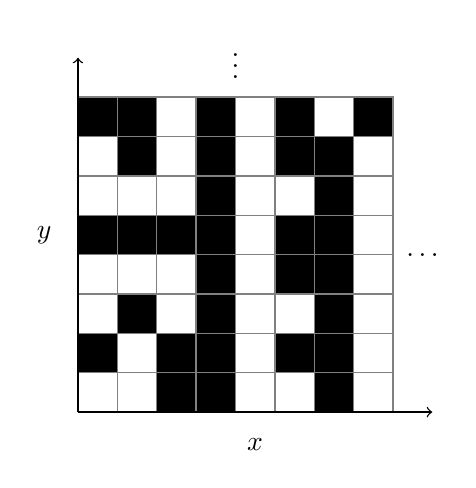
\begin{tikzpicture}[line width =0.5pt, scale=0.5]

\draw[gray] (0,0) grid (8,8);
\foreach \x/\y in {0/1, 0/4, 0/7, 1/2, 1/4, 1/6, 1/7, 2/0, 2/1, 2/4, 3/0, 3/1, 3/2, 3/3, 3/4, 3/5, 3/6, 3/7, 5/1, 5/3, 5/4, 5/6, 5/7, 6/0, 6/1, 6/2, 6/3, 6/4, 6/5, 6/6, 7/7}
    \filldraw[fill=black, draw=gray] (\x,\y) rectangle ++(1,1);
\draw[->] (0,0) -- (9,0) node[midway, below=6pt]{$x$};
\draw[->] (0,0) -- (0,9) node[midway, left=6pt]{$y$};
\node[] at (4,9){$\vdots$};
\node[] at (8.75,4){$\dots$};
\end{tikzpicture}
        %\caption{Infinite checkerboard with the square $(x,y)$ shaded iff $P(x,y)$ (for some arbitrary $P(x,y)$)}
        \label{fig:checkerboard1}
    \end{subfigure}\hfill%
    \begin{subfigure}{0.45\textwidth}
        \centering
        \usetikzlibrary{arrows}
\usetikzlibrary{positioning}

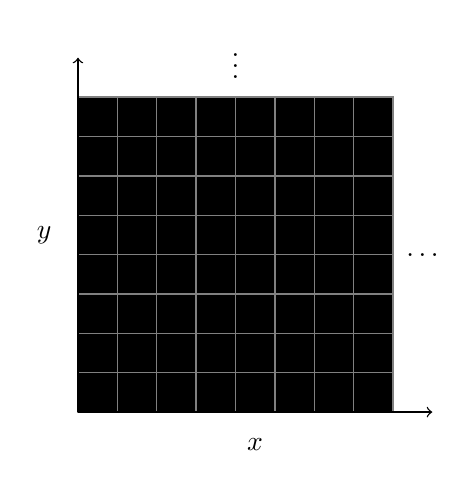
\begin{tikzpicture}[line width =0.5pt, scale=0.5]

\draw[gray] (0,0) grid (8,8);
\foreach \x in {0, 1, 2, 3, 4, 5, 6, 7}
    \foreach \y in {0, 1, 2, 3, 4, 5, 6, 7}
        \ifthenelse{\x<\y}{\def\col{white}}{\def\col{black}}
        \filldraw[fill=\col, draw=gray] (\x,\y) rectangle ++(1,1);

\draw[->] (0,0) -- (9,0) node[midway, below=6pt]{$x$};
\draw[->] (0,0) -- (0,9) node[midway, left=6pt]{$y$};
\node[] at (4,9){$\vdots$};
\node[] at (8.75,4){$\dots$};
\end{tikzpicture}
        %\caption{Infinite checkerboard with the square $(x,y)$ shaded iff $P(x,y)$ (where $P(x,y):=x\ge y$}
        \label{fig:checkerboard2}
    \end{subfigure}
    \caption{Shading $P(x,y)$ as a checkerboard, the $\Sigma_2$ sentence $\exists x,\forall y, P(x,y)$ can be interpreted as ``there is an infinite black column''. Left: an arbitrary example; Right: the example of $P(x,y):=x\ge y$, where the $\Sigma_2$ sentence is false, yet it is true for every ``finite window''.}
    \label{fig:checkerboard}
\end{figure}

Instead in this paper, we propose a game-theoretic solution relying on a slightly modified version of Hintikka's Verification-Falsification (VF) game \cite{hintikkaGameTheoreticSemantics1997}, the crucial difference being that players' moves are in $\finset{\Nats}$ rather than $\Nats$ itself.

\begin{definition}[Verification-Falsification game]
    To each FOL sentence $P$ we associate a game between two players, the ``Verifier'' and the ``Falsifier''. If $P$ is $\Delta_0$, then the Verifier or Falsifier win \$1 if $P$ is true or false respectively. Else if $P$ is $\Sigma$, the Verifier goes first and if $P$ is $\Pi$, the Falsifier goes first. The first player chooses $S\in\finset{\Nats}$ as their first move, and the game proceeds as the VF game for $\play{P}{S}$.
    \label{def:vfgame}
\end{definition}

The idea is then as follows: \emph{we measure how much traders are willing to pay to play the Verification-Falsification game for some sentence $P$}. Another way of expressing this is: the asset for some sentence $\exists x,P(x)$ is the \emph{option} to exchange it for any $\bigvee_{x\in S}P(x)$ for $S$ finite; while $\forall x,P(x)$ is the \emph{obligation} to exchange it for any $\bigwedge_{x\in S}P(x)$ chosen by the opponent.

As we know from \ref{lem:nogo}, this framework does not have the standard property that agents are incentivized to bet sentences up to their subjective probability. In particular, we see that an agent's fair price in this game not only depends on its belief in the statement, but its ability to construct specific values for the bound variables to win the game. Still, we may construct a theoretical program market for our framework that has at least some closely related desirable properties.

\begin{definition}[Prediction Market for VF games]
    Define the following:
    \begin{itemize}
        \item A \emph{price setter} $\agent[p]$ is composed of:
        \begin{itemize}
            \item a \emph{price sequence} $\price[p]:t\mapstopt\Props\too\probs$
            \item a \emph{player} $\player[p]:t\mapstopt\Props\too\strings\too\moves$
            \item a \emph{labeler} $\labeler[p]:t\mapstopt\Props\too\Rats\toe\maybe{\strings}$ such that $\intlen{\supp{\labeler[p](t,P)}}=\inventory[m](t,P)$ (defined by mutual recursion below)
        \end{itemize}
        \item An \emph{agent} $\agent$ is composed of:
        \begin{itemize}
            \item an \emph{endowment} $\endowment\in\Rats$ and a \emph{birthday} $\birthday\in\Nats$
            \item a \emph{trader} $\trader:t\mapstopt\Props\too\probs\tode\Rats$
            \item a \emph{player} $\player:t\mapstopt\Props\too\strings\too\moves$
            \item a \emph{labeler} $\labeler:t\mapstopt\Props\too\Rats\toe\maybe{\strings}$ such that $\intlen{\supp{\labeler(t,P)}}=\inventory(t,P)$ (defined by mutual recursion below)
            \item an \emph{inventory} $\inventory:t\mapstopt \Props\too\Rats$ defined by (initial conditions) $\inventory(s,\top)=0$ for $s<\birthday$, $\inventory(\birthday,\top)=\endowment$ and for all other propositions $\inventory(0,P)=0$ and (recursion rule) $\inventory(t+1)=\inventory(t)+\sum_{P,i}\change[P,i](t)$ where:
            \begin{itemize}
                \item orders placed: $\change[P,1](t,P)=\lambda\trader(t,P,\price(t,P))$ where $\lambda$ is 1 if the following conditions are met (else 0): for all $P$, $\max_p-\trader(t,P,p)\le \inventory(t,P)$ (you're not selling what you don't have) and $\sum_P\max_p p\trader(t,P,p)\le\inventory(t,\top)$ (you can afford all your purchases)
                \item cost of orders placed: $\change[P,2](t,\top)=-\price(t,P)\change[P,1](t,P)$
                \item the moves played (if $P\in\Sigma$): $\change[P,3](t,P)=-\sum_{l\in\supp{\player(t,P)}}{\intlen{\preimg{\labeler(t,P)}{l}}}$ and $\change[P,4](t,\play{P}{\player(t,P,l)})=\intlen{\preimg{\labeler(t,P)}{l}}$
                \item the opponent's moves (if $P\in\Pi$): $\change[P,5](t,P)=-\sum_{l\in\supp\player(t,P)}{\intlen{\preimg{\labeler[p](t,P)}{l}}}$ and $\change[P,6](t,\play{P}{\player[p](t,P,l)})=\intlen{\preimg{\labeler[p](t,P)}{l}}$
                \item the payout from empirical truth (if $P\in\Delta_0$): if $P\in\supp\xi(t)$, then $\change[P,7](t,P)=-\inventory(t,P)$ and $\change[P,8](t,\xi(t,P))=\inventory(t,P)$
            \end{itemize}
        \end{itemize}
        \item the \emph{empirical reality} is a process $\xi:t\mapstopt\Delta_0\too\maybe{\Bools}$ such that $s\le t,P\in\supp\xi(s)\implies\xi(t,P)=\xi(s,P)$ and $\bigcup_t\supp\xi(t)=\Delta_0$ and $\xi(t,\lnot P)=\lnot\xi(t,P)$
        \item The type of agents is denoted as $\agent[s]:=\endowment[s]\times\birthday[s]\times\trader[s]\times\player[s]\times\labeler[s]$ where the respective types are already as specified (including sub-typing by the requisite condition); define specifically $\tpler:=\trader[s]\times\player[s]\times\labeler[s]$.
        \item The \emph{father of agents} is an enumerator and allocator for agents, i.e. a map $\father:t\mapsto\agent[s]$ such that $\proj[\tpler]\circ\father$ is bijective; the total endowment is finite $\sum_t{\endowment[\father(t)]}<\infty$; and the birthdays are correct $\birthday[\father(t)]=t$. It is associated with an \emph{aggregate agent} as follows:
        \begin{itemize}
            \item $\endowment[m]=\sum_t{\endowment[\father(t)]}$ and $\birthday[m]=0$
            \item $\trader[m](t)=\sum_{\agent=\father(1),\dots\father(t)}\lambda_{\agent}\trader(t)$ where $\lambda_{\agent}$ is 1 if the following conditions are met (else 0): for all $P$, $\max_p-\trader(t,P,p)\le\inventory(t,P)$ and $\sum_P{\max_{p}{p\trader(t,P,p)}}\le\inventory(t,\top)$ (this sum is only a finite sum, because only finitely many agents have any cash at $t$)
            \item $\player[m](t,P,\concat{\code{\agent}}{l})=\player(t,P,l)$ where $\code{\agent}$ indicates some encoding for agents
            \item $\labeler[m](t,P,q)=
            \begin{cases}
                \concat{\father(t_q)}{\labeler[\father(t_q)](t,P)} & \text{if }t_q\le t \\
                \zero & \text{else}
            \end{cases}$ \\
            where $t_q$ is the smallest value such that $\sum_{s\le t_q}{\inventory[\father(s)](t,P)}\ge q$, if it exists, else $\infty$.
        \end{itemize}
        \item A special price setter $\agent[pp]$, called \emph{equilibrium}, is defined as follows -- for each $t$ and $P$:
        \begin{itemize}
            \item $\price[pp](t,P)$ is any solution $p$ to $\trader[m](t,P,p)-\trader[m](t,\lnot P,1-p)=0$.
            \item $\player[pp](t,P)=\player[m](t,\lnot P)$
            \item $\labeler[pp](t,P)=\labeler[m](t,\lnot P)$
        \end{itemize}
    \end{itemize}
    \label{def:vfmarket}    
\end{definition}

A more readable description: each agent manages its \emph{inventory} $\inventory(t):\Props\too\Rats$; in particular $\inventory(t,\top)$ denotes an agent's cash reserves. At each point in time, $\trader(t,P)$ denotes its demand (or supply, if negative) schedule for $P$, which is a sum of limit orders. The description of the player has some subtle considerations: (1) the moves are in $\moves$ rather than $\finset\Nats$, because the move $\zero$ is interpreted as ``pass'', i.e. should the agent wishes to not instantly play his move when he acquires $P$ but compute his move over several time-steps (2) an agent that holds multiple stocks of some sentence might not want to play the same move on all of them.

We capture this behaviour by having the agent \emph{labelling} different portions of his inventory of stock $P$ with different labels, i.e. a labelled partition $\Rats\toe\maybe{\strings}$ of $\Rats$ so that only a fragment of $\Rats$ whose length equals the agent's stock in $P$ is mapped to a label, everything else is mapped to $\zero$. When $\player$ then plays a move for sentence $P$ and label $l$, the amount of $P$ stocks labelled with $l$ will be removed from the inventory and replaced with $\play{P}{\player(t,P,l)}$. 

In particular, the aggregate agent $\agent[m]$ uses this system to keep the inventories for different agents separate by prefixing their labels with some code for each agent as $\concat{\code{\agent}}{l}$ -- this is necessary for the crux of the program market concept, which is that each agent can only trade with its own money, so more successful agents gain influence (in the form of wealth) while those that go bankrupt are effectively removed from the market. This is done through the indicator denoted by $\lambda_{\agent}$, which checks if $\agent$ can afford the trades it makes.

Finally, some notes regarding equilibrium calculation: in our framework, agents provide independent demand schedules for each sentence (i.e. a map $\Props\too(\probs\to\Rats)$, rather than a map $(\Props\too\probs)\to\Rats$): in other words, should the agents wish for cross-elasticity in their demand-schedules, the onus is on them to estimate the prices of other sentences. This reduces equilibrium calculation to finding the zero of a non-increasing piecewise-constant function, which is elementary. The equilibrium price setter's player is more subtle: at equilibrium price, $\agent[m]$ buys equal amounts of $P$ and $\lnot P$, however it may use different players for different portions of each. So we have $\player[pp]$ use $\agent[m]$'s players for $\lnot P$ against $\agent[m]$'s players for $P$ and vice versa so it wins exactly as many games as it loses, as illustrated in Fig~\ref{fig:matchup}.

\begin{figure}
    \centering
    \usetikzlibrary{arrows}
\definecolor{aqaqaq}{rgb}{0.65,0.65,0.65}
\begin{tikzpicture}[line width =1pt]%[line cap=round,line join=round,>=triangle 45,x=1cm,y=1cm]
%\clip(-2.5,-2.15) rectangle (9.7,5.1);

\draw (-2.5,0.32) node[anchor=north west] {$\mu\text{'s labels}$};

\draw (0,0) -- (4,0) node[midway, below = 10pt]{$P$};
\draw [|-] (0,0) -- (1.2,0) node[midway, above]{$\small\tilde{\alpha}_1$};
\draw [|-] (1.2,0) -- (2.5,0) node[midway, above]{$\small\tilde{\alpha}_2$};
\draw [|-] (2.5,0) -- (3.1,0) node[midway, above]{$\small\tilde{\alpha}_3$};
\draw [|-|] (3.1,0) -- (4,0) node[midway, above]{$\small\tilde{\alpha}_4$};

\draw (5,0) -- (9,0) node[midway, below = 10pt]{$\lnot P$};
\draw [|-] (5,0) -- (5.7,0) node[midway, above]{$\small\tilde{\beta}_1$};
\draw [|-] (5.7,0) -- (6.9,0) node[midway, above]{$\small\tilde{\beta}_2$};
\draw [|-|] (6.9,0) -- (9,0) node[midway, above]{$\small\tilde{\beta}_3$};

\begin{scope}[color = aqaqaq]
\draw (-2.5,2.82) node[anchor=north west] {$\varpi\text{'s labels}$};

\draw [|-] (0,2.5) -- (0.7,2.5) node[midway, above]{$\small\tilde{\beta}_1$};
\draw [|-] (0.7,2.5) -- (1.9,2.5) node[midway, above]{$\small\tilde{\beta}_2$};
\draw [|-|] (1.9,2.5) -- (4,2.5) node[midway, above]{$\small\tilde{\beta}_3$};

\draw [|-] (5,2.5) -- (6.2,2.5) node[midway, above]{$\small\tilde{\alpha}_1$};
\draw [|-] (6.2,2.5) -- (7.5,2.5) node[midway, above]{$\small\tilde{\alpha}_2$};
\draw [|-] (7.5,2.5) -- (8.1,2.5) node[midway, above]{$\small\tilde{\alpha}_3$};
\draw [|-|] (8.1,2.5) -- (9,2.5) node[midway, above]{$\small\tilde{\alpha}_4$};

\draw [->] (6,1) -- (3,2);
\draw [->] (3,1) -- (6,2);
\end{scope}

\end{tikzpicture}
    \caption{Illustration of $\varpi$'s player countering $\mu$}
    \label{fig:matchup}
\end{figure}

\begin{definition}[Exploitation]
    An agent $\agent$ is said to \emph{exploit} a price-setter $\agent[p]$ if $\{\inventory(t,\top):t\in\Nats\}$ is bounded from below but not bounded from above.
    \label{def:exploit}
\end{definition}

\begin{lemma}[Inexploitabity]
    There is no agent $\agent\in\agent[s]$ that exploits $\agent[pp]$.
    \label{lem:inexploit}
\end{lemma}
\begin{proof}
    If any $\agent\in\agent[s]$ exploits $\agent[pp]$, then so does $\agent[m]$ (because the inventory allocated to $\agent$ will increase without bound, while all other agents' inventories are bounded below by 0 since they can only spend from their alloted inventory). However, by construction, $\agent[m]$ does not exploit $\agent[pp]$ (as it always holds an equal number of $P$ and $\lnot P$ stocks, and wins exactly as many games as it loses). Thus, no $\agent\in\agent[s]$ exploits $\agent[pp]$.
\end{proof}

\begin{theorem}[Convergence]
    $\lim_{t\to\infty}\price[pp](t,P)$ exists for all $P$; denote this as $\longrun(P)$.
    \label{thm:convergence}
\end{theorem}
\begin{proof}
    Suppose it didn't; then there exists $x\in(0,1)$ and $\varepsilon>0$ such that $\price[pp](t,P)>x+\varepsilon$ infinitely often and $\price[pp](t,P)<x-\varepsilon$ infinitely often. Then consider an agent given by a trader that sells when $\price[pp](t,P)>x+\varepsilon$ and buys when $\price[pp](t,P)<x-\varepsilon$, and a trivial player (doesn't play at all; returns $\zero$ each time). This agent exploits the market.
\end{proof}

Ideally, we would like to say that our market learns to correctly price very FOL sentence: that $P$ is equivalent to $\longrun(t,P)=1$, and $\lnot P$ is equivalent to $\longrun(t,P)=0$: because if a true sentence did not approach \$1, an agent could buy arbitrarily large quantities of it and win the VF game on them. However, we know from Lemma~\ref{lem:nogo} that this is impossible: indeed, the flaw in our intuition is that the mere existence of a winning strategy (i.e. the ``truth'' of $P$) does not imply it is actually computable. Instead, we adopt the following ``constructivist'' notion of truth, closely related to the notion of ``CGTS-truth'' (``Computational Game Theoretic Semantics Truth'') proposed in \cite{boyerProofTruth2012b}.

\begin{definition}[Constructive truth]
    Denote $\instaplayer[s]:=\Props\toc\finset\Nats$. For any $P\in\Props$ and $\instaplayer,\instaplayer[b]\in\instaplayer[s]$, observe that the sequence $\play{P}{\instaplayer,\instaplayer[b],\instaplayer,\instaplayer[b],\dots}$ eventually converges to a $\Delta_0$ sentence: denote this sentence by $\playfull(P,\instaplayer,\instaplayer[b])$. Then an FOL-sentence $P$ is said to be $\instaplayer[s]$-true if $\exists\instaplayer\in\instaplayer[s],\forall\instaplayer[b]\in\instaplayer[s],\playfull(P,\instaplayer,\instaplayer[b])$, and $\instaplayer[s]$-false if $\exists\instaplayer[b]\in\instaplayer[s],\forall\instaplayer[a]\in\instaplayer[s],\lnot\playfull(P,\instaplayer,\instaplayer[b])$.
    \label{def:constructive}
\end{definition}

\begin{lemma}[Correspondence between $\instaplayers$ and $\players$]
    For any $\instaplayer:\Props\toc\finset\Nats$ there is a corresponding $\player:t\mapstopt\Props\too\strings\too\moves$ that executes it,, such that the following conditions are met: (1) $\forall s\ne t,\supp\instaplayer(t)\cap\supp\instaplayer(s)=\varnothing$ and (2) if $P\in\supp\instaplayer$ ($\instaplayer$ halts on input $P$) then $\exists t,\player(t,P,\foo)=\instaplayer(P)$ else $\forall t,\player(t,P,\foo)=\zero$.
    \label{lem:correspondence}
\end{lemma}
\begin{proof}
    Fix an enumeration of $\Props$ i.e. a bijection $\zeta:\Nats\to\Props$, and fix a model of computation for $\instaplayer$, e.g. a Turing Machine. Then define $\player$ as follows:
    \begin{equation*}
        \player(t,P,l)=
        \begin{cases}
            \instaplayer(P) & \text{if } P\in\{\zeta(0),\dots,\zeta(t)\},\\&\ \ \ %
            \halts(\instaplayer,P,t),\\&\ \ \ \:% 
            l=\foo \\
            \zero & \text{else}
        \end{cases}
    \end{equation*}
\end{proof}

\begin{theorem}[Learning constructive truth]
    If $P$ is an $\instaplayer[s]$-true sentence, then $\longrun(P)=1$. 
    \label{thm:main}
\end{theorem}
\begin{proof}
    Suppose it wasn't; then there is some $\varepsilon$ such that $\price[pp](t,P)$ is below $1-\varepsilon$ infinitely many times. Then consider the agent given by (1) the trader $\trader$ that buys whenever $\price[pp](t,P)<1-\varepsilon$ (2) the player $\player$ that is the Lemma~\ref{lem:correspondence}-correspondent of the $\instaplayer$ affirmed in the hypothesis $\exists\instaplayer\in\instaplayer[s],\forall\instaplayer[b]\in\instaplayer[s],\playfull(P,\instaplayer,\instaplayer[b])$ (3) the labeler $\labeler$ that returns $\foo$ on all outputs. This agent exploits the market.
\end{proof}

\begin{corollary}[Learning constructive falsehood]
    If $P$ is an $\instaplayer[s]$-false sentence, then $\longrun(P)=0$.
    \label{cor:main}
\end{corollary}
\begin{proof}
    Apply Thm~\ref{thm:main} to $\lnot P$.
\end{proof}

\section{Concluding remarks}

\subsection{Future work}

There are several research directions available to me based on the work I've done so far, broadly categorized as follows:

\begin{enumerate}
    \item \textbf{The main project} -- i.e. latent space markets, as described as RQ2 in the introduction.
    \item \textbf{Interpretability} -- i.e. mechanisms to incentivize agents to make bets on each others' latent spaces, as described as RQ3 in the introduction and as motivated by the discussion on \cite{christianoElicitingLatentKnowledge2021}.
    \item \textbf{Coherent extrapolated volition (CEV)} -- One crucial observation underlying my project is that program markets naturally capture the notion of \emph{rationality conditioned on algorithmic information}. \cite{yudkowskyCoherentExtrapolatedVolition2004} asks what an agent would look like with ``unlimited algorithmic information''; program markets may be the right framework to model this problem. 
    \item \textbf{Practical markets for FOL sentences} -- Building real-world prediction markets for FOL sentences (e.g. prediction markets for various practically relevant statistical questions may be expressed in terms of limiting distributions of experimental results, thus as $\Pi_3$ sentences). With practical markets, however, special attention must be taken to take into account asymmetries in the computational costs of players for opposing sides: in our theoretical framework, every possible player was enumerated in the market, however practically some players may be ``more expensive'' than others, and this may influence how much traders are willing to pay for a side. For example, this may be addressed by ``separating out'' the market for players from the prediction market, so that traders are explicitly paying a price for purchasing players and this price can be added to the probability estimate for a sentence. In particular, this might also make it feasible to implement such systems with an automated market maker (e.g. logarithmic market scoring \cite{hansonLogarithmicMarketScoring2002, hansonCombinatorialInformationMarket2003}), as the obstacle to doing this immediately with our framework is that it's not obvious what player such a market-maker would use. 
    \item \textbf{Implications for mathematical logic} -- One potential implication of my work in mathematical logic: it provides a new approach to measuring the strength of a mathematical theory: in a slightly modified version of game semantics that allows one player to ``go back and change its moves'' \cite{bonnayPreuvesJeuxSemantiques2004}, a formal proof from a mathematical theory may be understood as a computable strategy to this modified verification-falsification game \cite{boyerProofTruth2012b}; we my then consider the maximum wealth that can be acquired by an agent that only trades and plays in accordance with a theory, and regard this as a measure of the strength of the theory.
    \item\textbf{Game-theoretic probability} -- Our result (Thm~\ref{thm:main}) is still somewhat weak, in that it says nothing about sentences that are neither $\instaplayer[s]$-true nor $\instaplayer[s]$-false -- from Thm~\ref{thm:convergence}, we know that the market price of every sentence converges to \emph{something}, and it would be interesting to study the nature of this limiting distribution. It would not be a probability distribution in the traditional sense -- i.e. you would not have $\Prob[\exists x,P(x)]=\sup_x\Prob[\exists i\le x,P(i)]$ and $\Prob[\forall x,P(x)]=\inf_x\Prob[\forall i\le x,P(i)]$, as this would contradict Lemma~\ref{lem:nogo}. Instead we might consider an alternate definition of a $\sigma$-algebra which is required to be closed only under unions and intersections of \emph{computable sequences}, i.e. replacing the countable union axiom with ``$\psi:\Nats\toc\mathcal{F}\implies\bigcup_i\psi(i)\in\mathcal{F}$'' and adopting a suitable generalized notion of probability measure on this algebra. Possibly relevant work to this end includes: quantifier algebras \cite{cwooQuantifierAlgebra2013}, Shafer \& Vovk's game-theoretic formulation of probability theory \cite{shaferProbabilityFinanceIt2005, shaferGameTheoreticFoundationsProbability2019} and Japaridze's ``Computability Logic'' \cite{japaridzeBeginningWasGame2009, japaridzeSurveyComputabilityLogic2015}.
    \item \textbf{Bridges to neural networks} -- as it stands, program markets remain quite impractical; while I believe latent space markets will address this in part, it may also be worth investigating if any of our results could translate to existing AI architectures; \cite{wentworthCompetitiveMarketsDistributed2018}, which draws analogies between markets and neural networks, might be worth studying to this end.
\end{enumerate}
Of these, I should have the first two fully fleshed-out in a paper by the next annual review; the remaining are side-quests which I can initiate some work in, perhaps with some collaborators.

\subsection{Reflections}

\begin{events*}
    I attended the Co-operative AI Foundation's summer workshop in July 2023, where I presented a brief poster on my ideas and discussed them with some people working on related fields. 

    I'll probably submit my first paper to LOFT 2024 (Jul) or WINE 2024 (Dec) after a finishing touch. I'm also considering attending workships like SERI MATS and UC Berkeley SPAR to find potential collaborators, as my research is starting to open up several different opportunities that I cannot simultaneously focus on all at once.
\end{events*}

\begin{skills*}
    Generally speaking it has been quite exciting to see how closely my specific topic is related to so many other areas of interest to me, and my work has helped me gain a much more intimate familiarity with the literature in these areas. Two particular ``soft skills'' I've gotten better at are literature review and academic networking (the latter over the course of the CAIF workshop), two areas I've always been kinda sucky at. 
\end{skills*}

\begin{collaboration*}
    I generally have weekly meetings with my supervisor, and resort to emails when that is not possible. I do not have other collaborators as of yet, though I am seeking to expand on that.
\end{collaboration*}

\section*{Bibiliography}

\subsection*{Papers (drafts and publications)}
My framework for betting on FOL sentences \cite{abhimanyupallavisudhirBettingWhatNeither2023}.
\newrefcontext[labelprefix=O]
\printbibliography[filter=self]


\subsection*{Markets and information}
General introductions to prediction markets \cite{conitzerPredictionMarketsMechanism2012, hansonLogarithmicMarketScoring2002, hansonCombinatorialInformationMarket2003}.
\newrefcontext[labelprefix=MI]
\printbibliography[filter=predmarkets]

\subsection*{Program markets}
\cite{garrabrantLogicalInduction2016, oesterheldTheoryBoundedInductive2023} are the classical works on this; \cite{wentworthCompetitiveMarketsDistributed2018} describes a relationship between markets and neural networks; \cite{ baumModelIntelligenceEconomy1999, changDecentralizedReinforcementLearning2020, kweeMarketBasedReinforcementLearning2001} are similar works to \cite{oesterheldTheoryBoundedInductive2023}.
\newrefcontext[labelprefix=PM]
\printbibliography[filter=progmarkets]

\subsection*{Latent space}
\cite{christianoElicitingLatentKnowledge2021} lays out the ``Eliciting Latent Knowledge'' program for interpetability; the topic of prediction markets for latent space knowledge has been partially addressed in \cite{tailcalledLatentVariablesPrediction2023, baillonBayesianMarketsElicit2017, baillonSimpleBetsElicit2021}; Wentworth's work on natural abstractions \cite{wentworthRulesAlgebraBayes2023, johnswentworthNaturalLatentsMath2023} can be understood as introducing a logic or algebra for the latent space.
\newrefcontext[labelprefix=L]
\printbibliography[filter=latent]

\subsection*{Math}
Related math and formal logic I've consulted over the course of my work on FOL markets: \cite{wuppuluriUnravellingComplexityLife2019} on algorithmic complexity; \cite{shaferGameTheoreticFoundationsProbability2019, shaferProbabilityFinanceIt2005} discuss an alternate ``game-theoretic'' formulation of probability theory, something of that sort might be necessary to capture long-run prices of FOL sentences in my framework; \cite{hintikkaGameTheoreticSemantics1997, boyerProofTruth2012b, bonnayPreuvesJeuxSemantiques2004, japaridzeBeginningWasGame2009, japaridzeSurveyComputabilityLogic2015} address game semantics and computability logic.
\newrefcontext[labelprefix=M]
\printbibliography[filter=math]

\subsection*{Economics}
General discussion of computational costs in economics \cite{normanComputabilityComplexityEconomics1994, rustDealingComplexityEconomic1997, chenEfficiencyComplexityComputational1990}; on transaction costs \cite{barzelTransactionCostsAre1985}.
\newrefcontext[labelprefix=E]
\printbibliography[filter=econ]

\subsection*{Bounded rationality}
General overviews and discussion of bounded rationality \cite{simonModelsManSocial1957, gigerenzerBoundedRationalityAdaptive2002, gigerenzerRationalTheoryHeuristics2016, arrowBoundedRationalityUnboundedly2004}; Russell \& Subramanian's "bounded optimality" \cite{russellProvablyBoundedOptimalAgents1995, russellRationalityIntelligenceBrief2016}; Coherent Extrapolated Volition \cite{yudkowskyCoherentExtrapolatedVolition2004}; equilibriums of games between machines/programs \cite{halpernAlgorithmicRationalityGame2014, halpernDonWantThink2011, tennenholtzProgramEquilibrium2004, lewisComputationalRationalityLinking2014, zilbersteinMetareasoningBoundedRationality2011}; thermodynamic rationality \cite{ortegaInformationTheoreticBoundedRationality2015, ortegaInformationUtilityBounded2011, ortegaThermodynamicsTheoryDecisionmaking2013, gottwaldBoundedRationalDecisionMaking2019}.
\newrefcontext[labelprefix=BR]
\printbibliography[filter=br]

\subsection*{Lampposts for support}
Literature on relatively efficient outcomes arising from ``zero-intelligence'' traders, hinting in favour of my intuition that a market composed of many simple traders can lead to emergent intelligence \cite{godeAllocativeEfficiencyMarkets1993, godeWhatMakesMarkets1997, jamalSimpleAgentsIntelligent2015, laibsonSafetyMarketsImpossibility2007, schwartzHowMuchIrrationality2008}.
\newrefcontext[labelprefix=X]
\printbibliography[filter=lampposts]

\end{document}